\chapter{A deep dive into the compiler}
%\label{chapter:title}

% \emph{Adding source code to your report/thesis is supported with the package {\normalfont\texttt{listings}}. An example can be found below. Files can be added using {\normalfont\texttt{\textbackslash lstinputlisting[language=<language>]\{<filename>\}}}.}

% \begin{lstlisting}[language=Python]
% """
% ISA Calculator: import the function, specify the height and it will return a
% list in the following format: [Temperature,Density,Pressure,Speed of Sound].
% Note that there is no check to see if the maximum altitude is reached.
% """

% import math
% g0 = 9.80665
% R = 287.0
% layer1 = [0, 288.15, 101325.0]
% alt = [0,11000,20000,32000,47000,51000,71000,86000]
% a = [-.0065,0,.0010,.0028,0,-.0028,-.0020]

% def atmosphere(h):
%     for i in range(0,len(alt)-1):
%         if h >= alt[i]:
%             layer0 = layer1[:]
%             layer1[0] = min(h,alt[i+1])
%             if a[i] != 0:
%                 layer1[1] = layer0[1] + a[i]*(layer1[0]-layer0[0])
%                 layer1[2] = layer0[2] * (layer1[1]/layer0[1])**(-g0/(a[i]*R))
%             else:
%                 layer1[2] = layer0[2]*math.exp((-g0/(R*layer1[1]))*(layer1[0]-layer0[0]))
%     return [layer1[1],layer1[2]/(R*layer1[1]),layer1[2],math.sqrt(1.4*R*layer1[1])]
% \end{lstlisting}

\definecolor{light-green}{rgb}{0.5,1,0.5}
\definecolor{light-blue}{rgb}{0.5,0.5,1}
\definecolor{light-red}{rgb}{1,0.5,0.5}
\definecolor{light-yellow}{rgb}{1,1,0.5}
\definecolor{light-grey}{gray}{0.5}

For this section, rather than show every listing for the source and compile code, I will provide links to the excellent tool \url{dpu.dev} to follow along. This is a web-based tool that allows us to interactively explore how snippets of codes are compiled for DPUs.

\section{Comparison}
\label{annex:comparison}

We mentioned in section \ref{subsection:DTimplementation} a pointer trick. To follow along, check out \href{https://dpu.dev/#g:!((g:!((g:!((g:!((h:codeEditor,i:(j:1,lang:___c,source:'int+leq(float+a,+float+b)+%7B%0A++++return+a+%3C%3D+b%3B%0A%7D%0A'),l:'5',n:'0',o:'C+source+%231',t:'0')),k:37.5,l:'4',m:50,n:'0',o:'',s:0,t:'0'),(g:!((h:codeEditor,i:(j:2,lang:___c,source:'int+leq(float+aa,+float+bb)+%7B%0A++++int+a+%3D*(int*)%26aa%3B%0A++++int+b+%3D*(int*)%26bb%3B%0A++++if+(a+%3C+0+%26%26+b+%3C+0)%0A++++++++return+b+%3C%3D+a%3B%0A++++else%0A++++++++return+a+%3C%3D+b%3B%0A%7D%0A'),l:'5',n:'0',o:'C+source+%232',t:'0')),header:(),l:'4',m:50,n:'0',o:'',s:0,t:'0')),k:47.25848563968668,l:'3',n:'0',o:'',t:'0'),(g:!((g:!((h:compiler,i:(compiler:clang-2021-3,filters:(b:'0',binary:'1',commentOnly:'0',demangle:'0',directives:'0',execute:'1',intel:'0',libraryCode:'1',trim:'1'),lang:___c,libs:!(),options:'',source:1),l:'5',n:'0',o:'clang+12+for+DPU+(rel+2021.3.0)+(Editor+%231,+Compiler+%231)+C',t:'0')),header:(),k:62.5,l:'4',m:50,n:'0',o:'',s:0,t:'0'),(g:!((h:compiler,i:(compiler:clang-2021-3,filters:(b:'0',binary:'1',commentOnly:'0',demangle:'0',directives:'0',execute:'1',intel:'0',libraryCode:'1',trim:'1'),lang:___c,libs:!(),options:'',source:2),l:'5',n:'0',o:'clang+12+for+DPU+(rel+2021.3.0)+(Editor+%232,+Compiler+%232)+C',t:'0')),header:(),l:'4',m:50,n:'0',o:'',s:0,t:'0')),k:52.74151436031331,l:'3',n:'0',o:'',t:'0')),l:'2',m:100,n:'0',o:'',t:'0')),version:4}{bit.ly/3a3s3fK}.

Consider the following code for a float comparison:
\begin{lstlisting}[language=C]
int leq(float a, float b) {
    return a <= b;
}
\end{lstlisting}

We can see in line 4 of the compiler that this results in long, simulated float comparison.

Now let's bit-cast out inputs to integers.
\begin{lstlisting}[language=C]
int leq(float aa, float bb) {
    int a =*(int*)&aa;
    int b =*(int*)&bb;
    if (a < 0 && b < 0)
        return b <= a;
    else
        return a <= b;
}
\end{lstlisting}

We're now doing the comparison in 3 instructions! This works because an IEEE floating point number is encoded as 

\begin{figure}[h]
    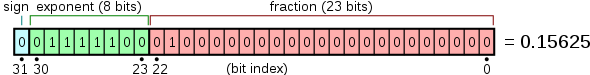
\includegraphics[width=0.7\textwidth]{figures/Float_example.svg.png}
    \caption[Float encoding.]{Float encoding.\footnotemark}
\end{figure}
\footnotetext{By Vectorization: Stannered - Own work based on: Float example.PNG, CC BY-SA 3.0, \url{https://commons.wikimedia.org/w/index.php?curid=3357169}}

So the conversion between a floating point and integer representation is monotonous (except for the inversion for negative 32 bits integers).

\section{Operands auto-promotion}
\label{annex:promotion}

In section \ref{subsection:Limitations}, we mentioned the limitations of the compiler when it comes to optimizing for our target architecture. We're now going to expose one such occurrence and how to deal with it. Follow along in \href{https://dpu.dev/#z:OYLghAFBqd5TKALEBjA9gEwKYFFMCWALugE4A0BIEAViAIzkA2AhgHagD63q5AzugCupVNhAByAKQAmAMwE2qJoJwBqSbIDCfIoTZEAdEg25JABgCC5iwqIA2ACyciq7IKUFMEW/TvOAVKos5Ko%2BfkSBAEYhgray0s6qfAQAXtgAlOoA7ABC1qoFofqOiSyoqIIAtoKsRNgaeZaFqgBmZBCx%2BvGJBBoAImYNoRraqfWyOcPSedOZkrn5zYVhiYQtLeqyfUGSAKw5vbvbALSqkXsHe30Ni0tB5VU1LHXq0/2qaxuBnzdNhfPXP4FUjYIjCNj3CrVWrjRpWLKAizidLMCS7cTkNgSMwY9ASTRJIQibCvWT0DFEbHIlEAaxAuzMqPEDgxlXpjKx4hx5Dx4gxfBAjMpXOR5DgsBQGBw%2BGIZEo1Do0mY7C4PH4RNEEhk8kUyjUIx0ekMxlkpks1lsJRcbg8XhWESCIXtURicQSLmSaTmCyBRXsThcZShTzqvwszTapA6bp6/UGE2GWk9sKmMxy3rhdwKADd0LUCEwSfaPgR1pttiwLocTmcq1cw1nIY8Ya88lsS2XvqWWg3/gjbqoQWDSBCg83nrDrADrKKmGiMZzubyCQJhKJSdIKVT0iikNgWDhSNQUXPmaz2ZiqTyJPzBeRhTid%2BQ6QymbIF1feVuRSjxQh4BAkroJUAAOBbYBQVAQBgoHgUeSgqsc0hmMhxyyOQLQFnUpAChAkRXpECgsKQACeEjkuQMGVNg%2BgAPJsEwZEiuQOCVCqhZXoQIKoEQBDZtgArMdgAAe2AVHU5EYrY2CntyTAEJEpDESRmhYGI4gUUQpAEGyGmziqIDcJwvDyZEAqQCi6Agbx6BsIJ/IamI9AnvOl7MbyCEcKo9BmK0ZCqH0AAKACqqgQCCTCqMhyEGLIBhmJkEAyiQpCkowqiqbBhapdqzkZd%2Bj60hep4suQbKvouuI3vwd4PqKf6AWgwFgdl8rQc1cFoKwHBIShZhoRhWEQbh%2BHMYRbDKZJlHAdRdEMUx3Ksex6mLQQ3G8fxgnciJYmCBJemUPoMlXqZSmkapOBTVpOmSSeBlGSZCnmRAlnWQQtn2eqa5iNILniOiblLhInnAN5vmRgFIVhRFUV9bF8WJcl/nakqGUddlG6ZJoBXUuQe4HhBx5MqV5Ucp%2B1UCkK25Fa%2Bp7voDVV8ve1NMpuDPXkzdVPvxOHvViDhAA}{bit.ly/39o9PFx}.

Consider the following code to compute a square euclidean distance between vectors \verb|a| and \verb|b|:
\begin{lstlisting}[language=C]
#include <stdint.h>

int64_t euclid(int16_t* a, int16_t* b, uint32_t size) {
    int64_t accumulate;
    for(uint32_t i=0; i<size; i++) {
        int16_t diff = a[i] - b[i];
        accumulate += diff * diff;
    }
    return accumulate;
}
\end{lstlisting}

What are we expecting to do here?
\begin{itemize}
    \item On line 6, we expect to compute the difference between two 16-bits coordinates and store it in a 16-bits integer. We know we can do that because we made sure our quantized coordinates fit in 15 bits.
    \item On line 7, we expect to compute the square of the difference ($16 \times 16 \to 32$) and accumulate it in a 64-bits integer.
\end{itemize}

But look at the compiler. There is a simulated 32-bits multiplication on line 17! The compiler coalesced lines 6 and 7. Since the compiler doesn't know that the subtraction won't overflow, it automatically promoted the subtraction result into a 32-bits integer. So now we're doing a $32 \times 32 \to 64$ multiplication.

This can be solved either by manually writing that part of the code in the assembler, or adding a \verb|volatile| qualifier to the \verb|diff| variable, preventing the compiler from optimizing it out. Now we have the $16 \times 16 \to 32$ multiplication we expected.

Do note that the C compiler does NOT perform such auto promotions between 32 and 64 bits variables, because the writers of the C standard were aware that it would lead programmers to make such mistakes on 32-bits processors. It's a simple fix, but the issue is so, so easy to miss.